\section{Introducción}
\subsection{Planteamiento del problema}

La robótica está cada vez más involucrada en el mercado laboral, lo que hace que la educación, en muchos casos, se quede corta para cubrir esta demanda. Por ello, se busca fomentar la inclusión de la robótica en diferentes niveles educativos: inspirando a los más jóvenes, introduciendo a los estudiantes en educación secundaria, y permitiendo que los más avanzados puedan profundizar en el área.

En este contexto, surge la necesidad de un modelo de brazo robótico accesible, fácil de ensamblar, de bajo costo y con un diseño sencillo que sea adecuado para usuarios inexpertos o jóvenes. Este modelo debe ser, además, duradero, mantenible y fácil de reparar, para garantizar su uso a largo plazo. Adicionalmente, se plantea que el manipulador sea modular, con la posibilidad de modificación y expansión, permitiendo a los estudiantes más avanzados involucrarse en proyectos más complejos y adaptarlos a otros sistemas o tecnologías.

La propuesta de utilizar MDF como material principal, aprovechando sus ventajas de bajo costo y facilidad de fabricación mediante corte láser o fresado CNC, busca superar las limitaciones que presentan los métodos de fabricación más lentos y costosos como la impresión 3D. De esta forma, se logra una producción más eficiente y replicable, accesible para más instituciones educativas.

El objetivo final es ofrecer un manipulador robótico que pueda adaptarse a diversas aplicaciones y demostraciones, fomentando el aprendizaje en robótica y automatización desde etapas tempranas de formación, inspirando a los estudiantes y acercándolos a los procesos industriales actuales.

\subsection{Diagrama de Ishikawa}

\vspace{1em}


\begin{figure}[h]
  \centering
  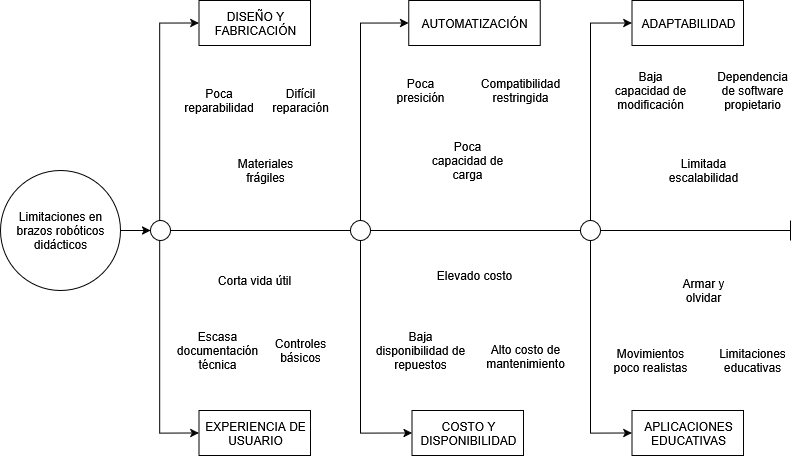
\includegraphics[width=0.8\textwidth]{anexos/Diagrama Ishikawa.png}
  \caption{Diagrama de Ishikawa (Fuente: elaboración propia)}\label{fig:Diagrama Ishikawa.}
\end{figure}
En el diagrama se identifican seis ramas principales que agrupan las limitaciones más comunes de los brazos robóticos didácticos disponibles en el mercado. Cada una de ellas aborda un conjunto de problemáticas específicas:
\begin{itemize}
  \item Diseño y fabricación: engloba aspectos relacionados con la construcción del brazo, los materiales empleados y la facilidad de reparación o mantenimiento.
  \item Automatización: considera las limitaciones en la precisión, capacidad de carga, compatibilidad y posibilidades de integración con otros sistemas de control.
  \item Adaptabilidad: se refiere a la capacidad de modificar, escalar o personalizar el brazo, así como a la dependencia de software propietario que restringe su flexibilidad.
  \item Experiencia de usuario: abarca las dificultades que enfrentan los usuarios en el manejo del brazo, tales como controles limitados, documentación insuficiente y vida útil reducida.
  \item Costo y disponibilidad: contempla el precio de adquisición, el costo de mantenimiento y la dificultad para conseguir repuestos o componentes compatibles.
  \item Aplicaciones educativas: analiza las limitaciones de los kits en contextos formativos, como la escasa realismo de los movimientos y el alcance reducido de sus usos pedagógicos.
\end{itemize}

\subsection{Solución propuesta}
Un brazo robótico didáctico a escala de 4 GDL con efector intercambiable: electroimán (para piezas ferromagnéticas) y garra (para piezas no magnéticas). Estructura paramétrica cortada en MDF (3.2–10 mm), tornillería estándar y electrónica de fácil reposición. Control con ESP32/ATmega328P, modos manual/automático, GUI en Python (Tkinter/PyQt), y documentación abierta para replicación.

\subsection{Objetivo General}
Desaroolar un modelo de brazo robótico didáctico de 4 grados de libertad, seguro, portable y accesible, con efectores electroimán/garra intercambiables, capaz de ejecutar tareas básicas de pick \& place en un volumen de trabajo de hasta 50×50×50 cm.

\subsection{Objetivos específicos}
\begin{enumerate}
  \item Diseñar la estructura mecánica del brazo robótico de 4 GDL en MDF paramétrico, asegurando su facilidad de ensamblaje, modularidad y bajo costo.

  \item Desarrollar un sistema de actuación con servomotores que permita manipular cargas de hasta 100 g en un alcance de 40 cm con una tasa de éxito superior al 90%.

  \item Implementar un sistema de efectores intercambiables (electroimán y garra) con un mecanismo de cambio rápido que no requiera herramientas especiales.

  \item Incorporar medidas de seguridad en el prototipo, incluyendo paro de emergencia, cableado protegido y tensiones seguras en la zona de usuario.

  \item Desarrollar una interfaz gráfica de usuario (GUI) que permita el control manual y automático del brazo, con funciones de lectura de posición, activación del electroimán y cinemática inversa planar.
\end{enumerate}


